\chapter{Related Work}
\label{chp:b2}

\section{HDR Imaging}

While HDR imaging has long been an active field of research, recent developments in HDR imaging~\cite{Rein2010,Banterle2011,chalmers2016high}, in particular those pertaining to HDR image and video capture~\cite{tocci2011versatile,froehlich2014creating} and display systems~\cite{seetzen2004high}, and HDR
video streaming standards~\cite{standard2016dynamic} to allow direct rendition of HDR images will likely make HDR images more common in the near future. However, despite the practical improvements in the field, there is also a need for fundamental and experimental research that explores various aspects related to HDR imaging and dynamic range. Hanhart et al.~\cite{hanhart2015benchmarking} investigated the performance of various objective metrics in quantifying visual distortions of HDR images commensurate with subjective opinions. Hanhart et al. found HDR-VDP-2~\cite{mantiuk2011hdr} and HDR-VQM~\cite{narwaria2015hdr} to be the best predictors of visual quality. In another study, Grimaldi et al.~\cite{grimaldi2019statistics} investigated how image statistics change as a function of dynamic range and found that there are indeed differences between HDR and LDR images. Grimaldi et al., also found, however, that the majority of these differences are accounted for by the early visual processing that takes place in the human visual system. Additionally, Rana et al.~\cite{rana2015evaluation} compared HDR and LDR images in terms of feature detection potential and showed that it is possible to extract more effective features from HDR images. However, these works do not consider the HDR image similarity problem.

\subsection{HDR Image Creation}
Standard camera sensors are not capable of capturing HDR images natively. Currently, there are several approaches to generate HDR images~\cite{banterle2017advanced}. The first approach is capturing HDR images directly with specialized HDR sensors~\cite{zhao2015unbounded}. Although there has been advancements on HDR sensors, these sensors are still under development and expensive. The second and the most commonly used method is combining multiple exposure images taken by a camera with a standard sensor. This method relies on using different exposure times to capture the details of different regions of the scene, longer exposure times for low luminance areas and shorter exposure times for brighter areas. Figure~\ref{fig:exposures} shows the images captured with different exposures of the same scene. This scene has a high dynamic range that is not possible to capture both the lower luminance (indoor) and higher luminance (garden) regions with a single exposure setting.

\begin{figure}
\begin{subfigure}[b]{0.33\textwidth}
    \centering
    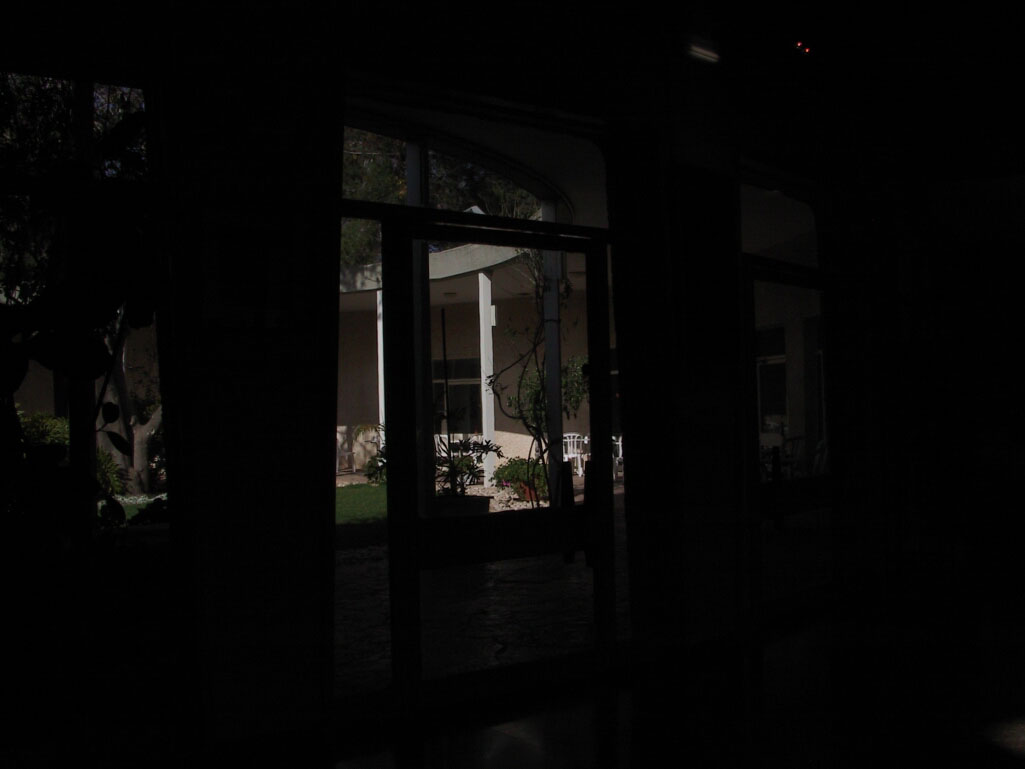
\includegraphics[width=\textwidth]{figures/chapter2/exposure/bh1.jpg}
    %\caption{Drago et al. ~\cite{drago2003adaptive}}
\end{subfigure}\hfill
\begin{subfigure}[b]{0.33\textwidth}
    \centering
    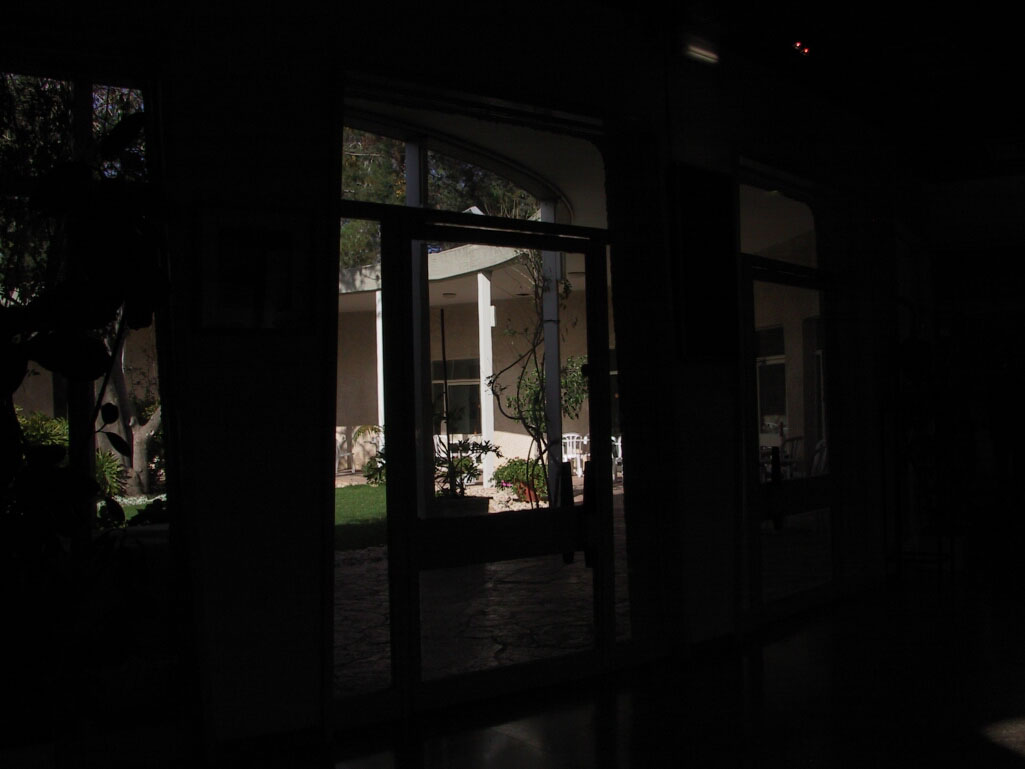
\includegraphics[width=\textwidth]{figures/chapter2/exposure/bh2.jpg}
    %\caption{Mai et al. ~\cite{mai2010optimizing}}
\end{subfigure}\hfill
\begin{subfigure}[b]{0.33\textwidth}
    \centering
    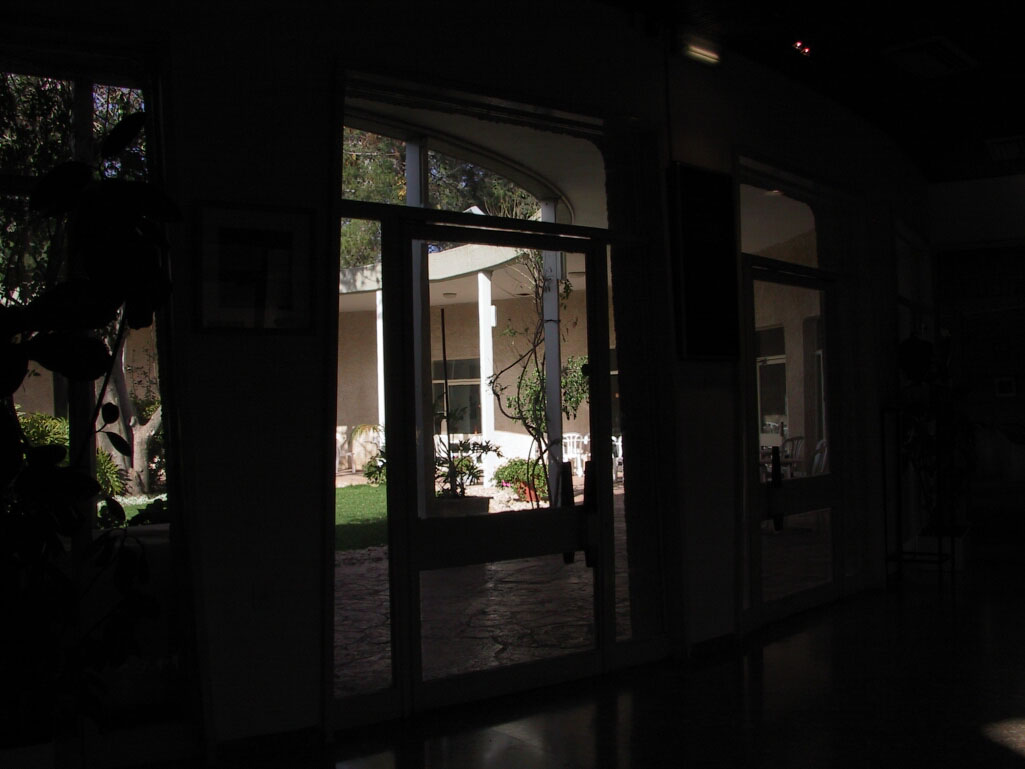
\includegraphics[width=\textwidth]{figures/chapter2/exposure/bh3.jpg}
    %\caption{Reinhard et al. (local) ~\cite{reinhard2002photographic}}
\end{subfigure}\\
\begin{subfigure}[b]{0.33\textwidth}
   \centering
    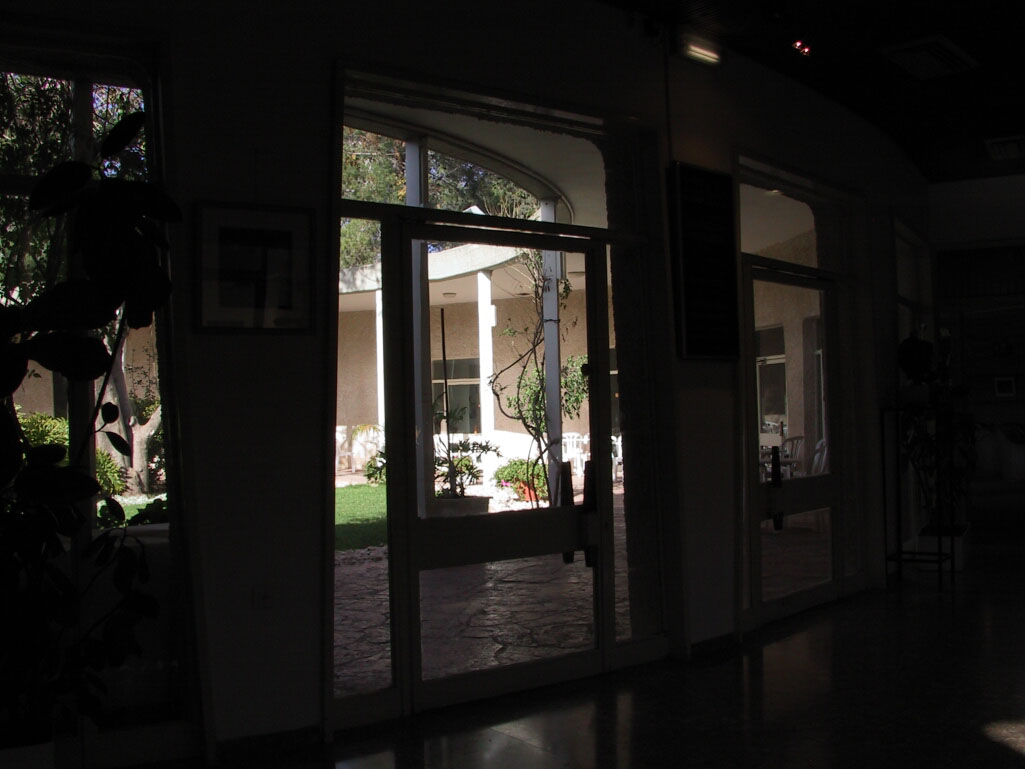
\includegraphics[width=\textwidth]{figures/chapter2/exposure/bh4.jpg}
    %\caption{Reinhard et al.(global) ~\cite{reinhard2002photographic}}
\end{subfigure}\hfill
\begin{subfigure}[b]{0.33\textwidth}
    \centering
    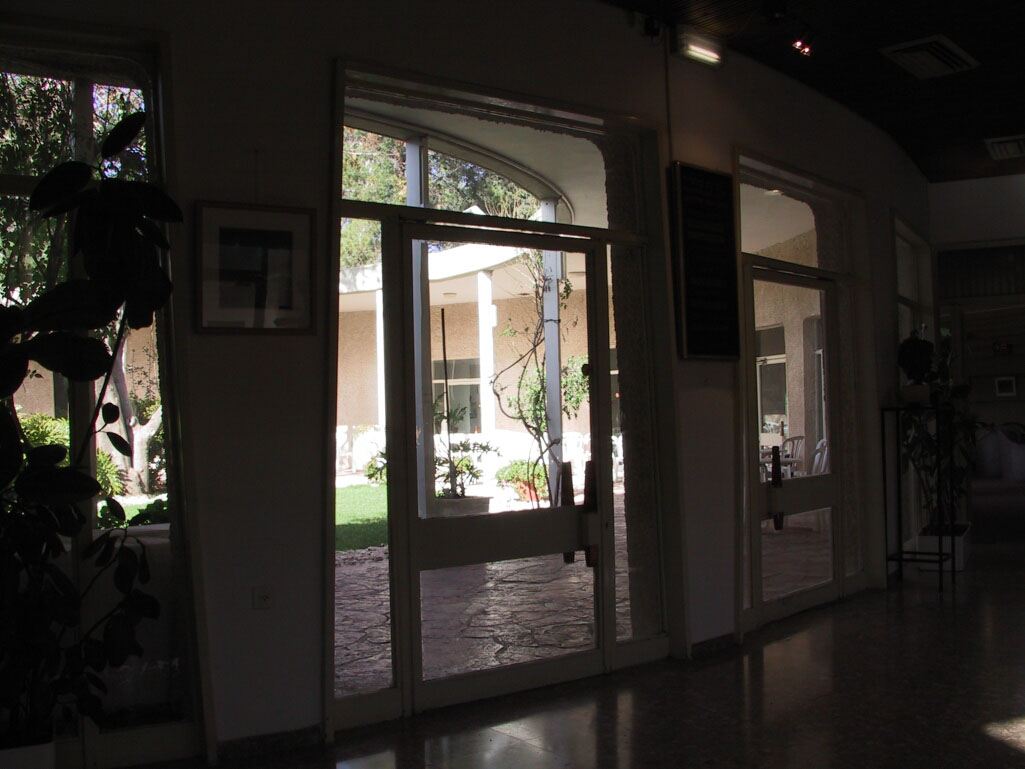
\includegraphics[width=\textwidth]{figures/chapter2/exposure/bh5.jpg}
    %\caption{Durand \& Dorsey~\cite{durand2002fast}}
\end{subfigure}\hfill
\begin{subfigure}[b]{0.33\textwidth}
    \centering
    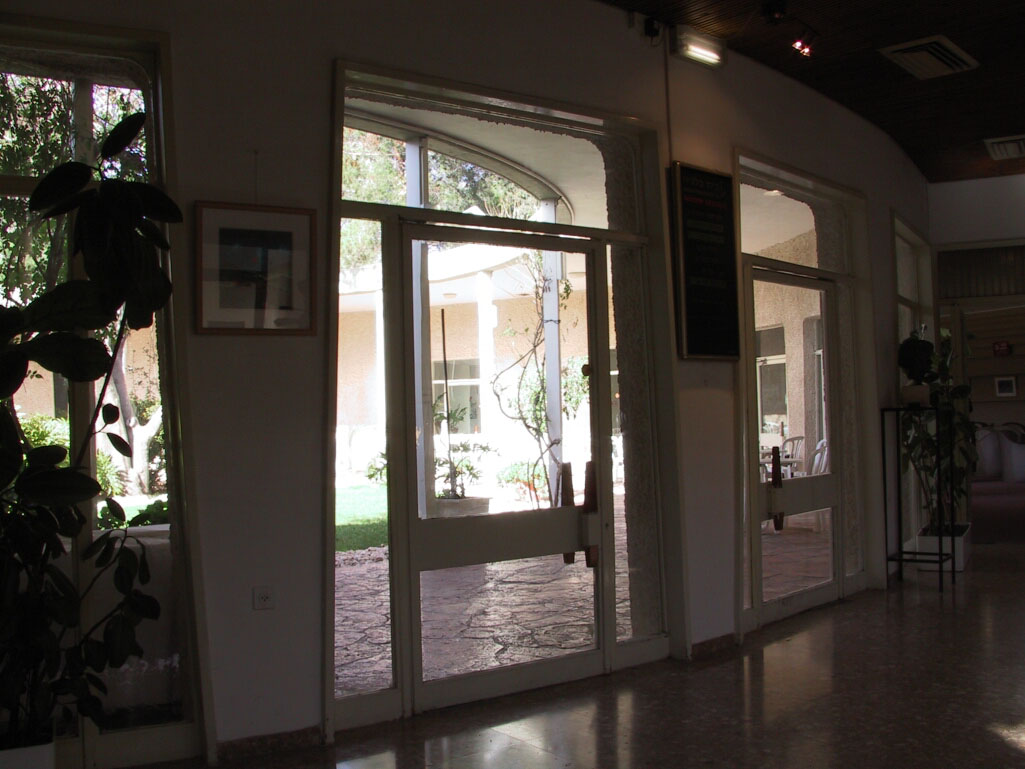
\includegraphics[width=\textwidth]{figures/chapter2/exposure/bh6.jpg}
    %\caption{Mantiuk et al.~\cite{mantiuk2006perceptual}}
\end{subfigure}\\
\begin{subfigure}[b]{0.33\textwidth}
    \centering
    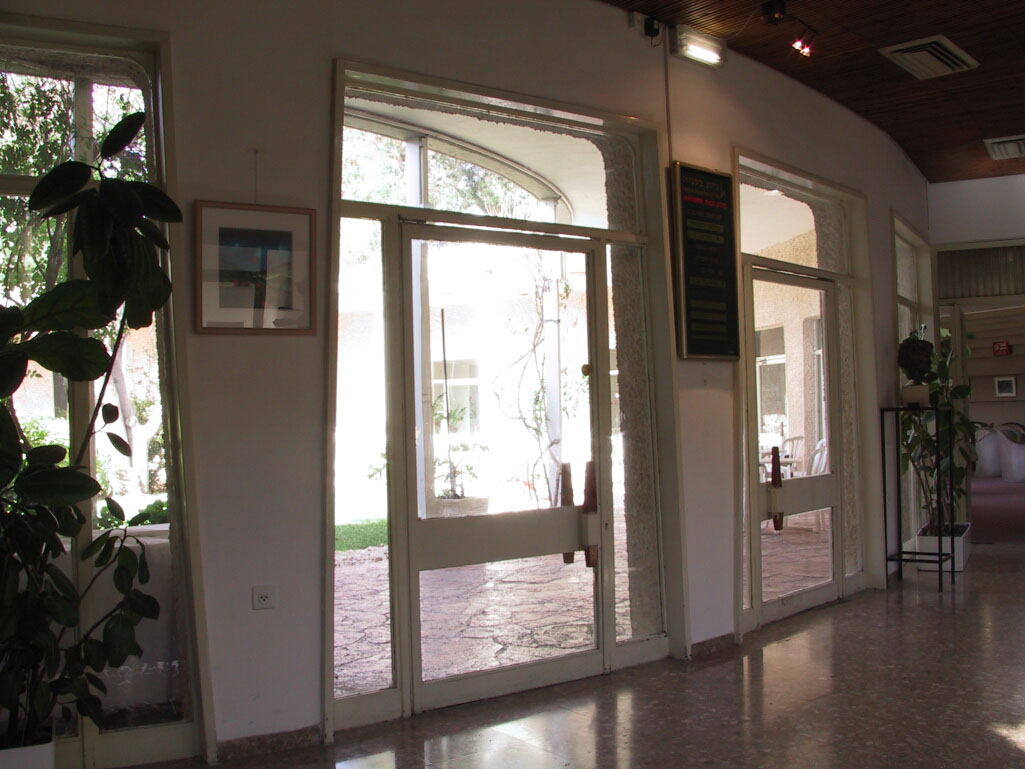
\includegraphics[width=\textwidth]{figures/chapter2/exposure/bh7.jpg}
    %\caption{Reinhard \& Devlin~\cite{reinhard2005dynamic}}
\end{subfigure}\hfill
\begin{subfigure}[b]{0.33\textwidth}
    \centering
    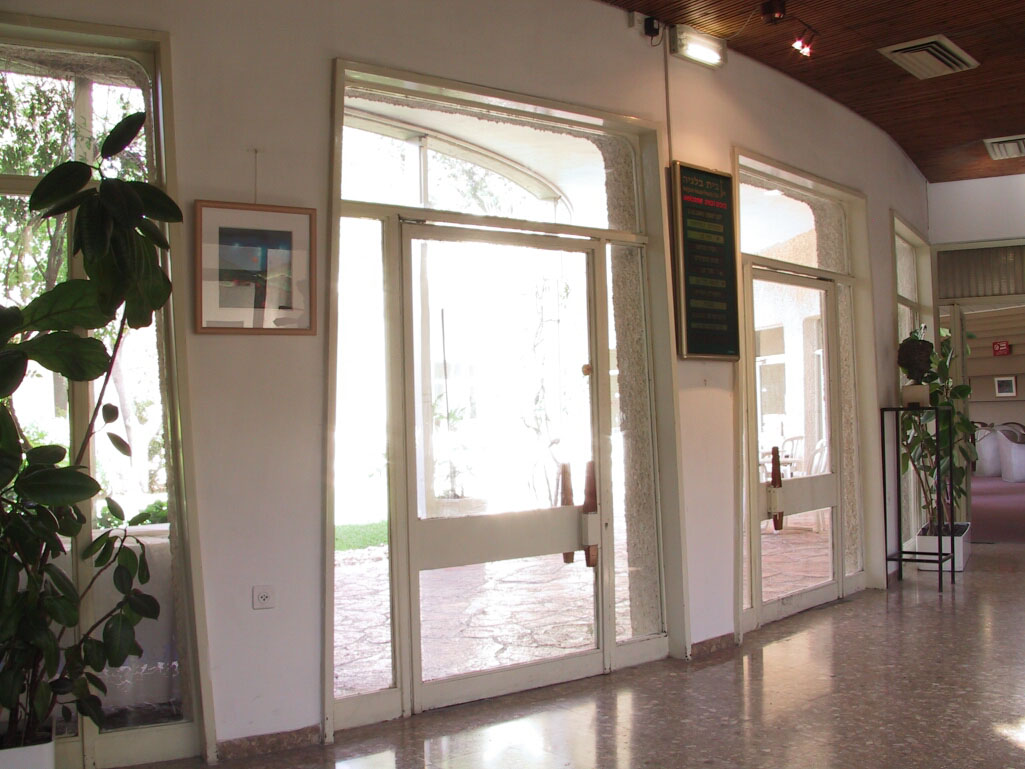
\includegraphics[width=\textwidth]{figures/chapter2/exposure/bh8.jpg}
    %\caption{Fattal et al.~\cite{durand2002fast}}
\end{subfigure}\hfill
\begin{subfigure}[b]{0.33\textwidth}
    \centering
    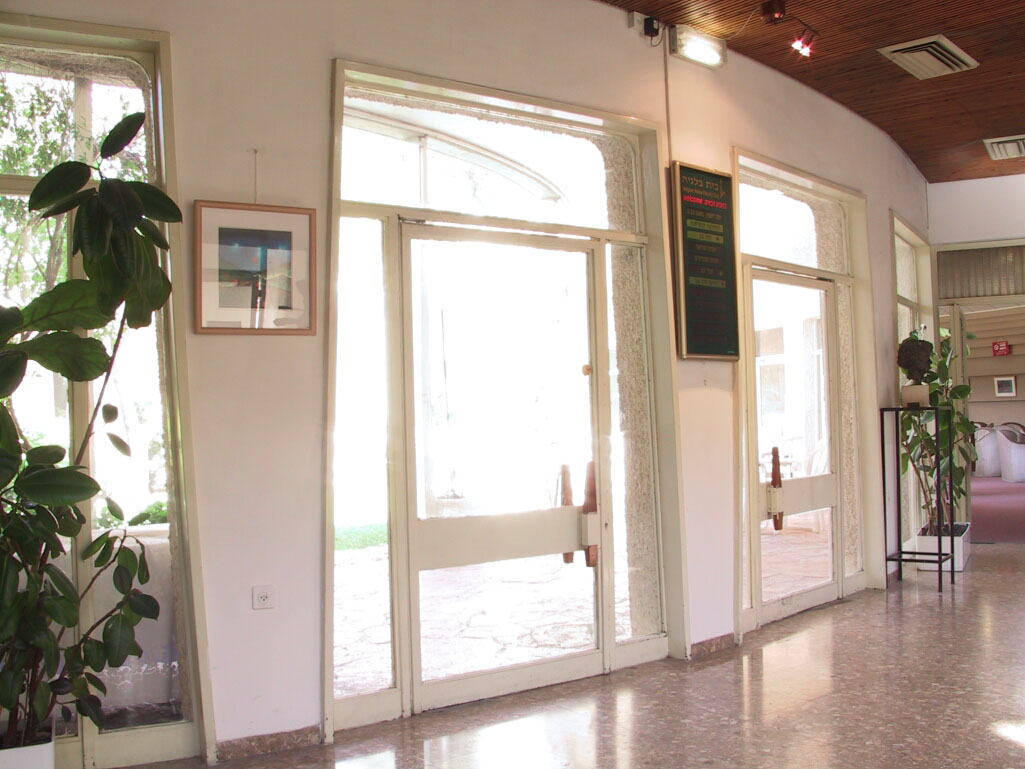
\includegraphics[width=\textwidth]{figures/chapter2/exposure/bh9.jpg}
    %\caption{Mantiuk et al.~\cite{mantiuk2008display}}
\end{subfigure}\hfill
\caption{"Belgium House" scene captured with different exposures (image courtesy of Dani Lischinski). }
\label{fig:exposures}
\end{figure}

After the series of images are captured with the same camera, it is possible to recover irradiance, $E$, for each pixel, $x$ with~\cite{banterle2017advanced}:

\begin{equation}
    E(x) = {{\sum^{N_e}_{i=1} w(I_i(x)) {I_i(x) \over \Delta t_i}} \over {\sum^{N_e}_{i=1} w(I_i(x))}} 
\end{equation}

where $I_i$ is the image captured with exposure $i$, $\Delta t_i$ is the exposure time, $N_e$ is the number of used exposures and $w$ is a weighting function to remove outliers. Note that camera response is assumed linear. For the cases that this assumption does not hold corrections need to be made. Dynamic scenes poses challenges for this approach, known as ghosting, and there are many deghosting algorithms to overcome this problem~\cite{Tursun2015_deghosting_survey}. The third approach is using a single camera with multiple sensors to capture different exposures of the same scene simultaneously~\cite{tocci2011versatile,mcguire2007optical}. However, these cameras are costly and hard to calibrate. The last approach to create HDR images is using a single LDR image and expanding the dynamic range approximately, known as inverse tone mapping. There are many studies on inverse tone mapping~\cite{akyuz2007hdr,masia2009evaluation,wang2007high,huo2014physiological} and this topic will gain more importance with the necessity of displaying LDR images on HDR displays arises as the usage of HDR displays increasing. Recently, there are also studies ~\cite{eilertsen2017hdr,metzler2020deep} that employs deep neural network based approaches for inverse tone mapping. 


\subsection{Tone Mapping}
HDR images can capture the true dynamic range of a scene by using wider representations compared to standard 8 bit images. However, in order to display or print HDR images on conventional devices, the dynamic range of the image should be compressed to match the dynamic range of the device. This operation, namely tone mapping, aims to compress the dynamic range while keeping the visual appearance intact. 

Tone mapping is an extensively studied research area and there are many tone mapping operators~\cite{Rein2010}. Comparison and subjective evaluation of the tone mapping operators is also an active research area~\cite{kundu2017large, krasula2016preference}. In this thesis, to investigate the effect of tone mapping operators to visual similarity, eleven commonly used tone mapping operators are selected. Basically, these tone mapping operators can be divided into three categories depending on their operation domain: global and local operators in spatial domain, and gradient domain operators~\cite{Rein2010}. 

Global tone mapping operators apply the same non-linear function to all luminance values without considering pixel neighbourhood. This makes these operators fast compared to other tone mapping operators however, they may result with contrast loss in dark and bright regions. Reinhard et al.~\cite{reinhard2002photographic} introduces a transfer function that compresses low luminance values less and high luminance values more. Drago et al.~\cite{drago2003adaptive} uses logarithmic compression for tone mapping while adaptively changing the logarithm base depending on the luminance value. A global algorithm is proposed by Pattanaik et al.~\cite{pattanaik2000time}, which takes in to account the illumination adaptation time of HSV. Other global methods that model photoreceptors of HVS is the work from Reinhard \& Devlin ~\cite{reinhard2005dynamic} and Ferradans et al.~\cite{ferradans2011analysis}. Mantiuk et al.~\cite{mantiuk2008display} models the display as well as HSV. On the other hand, Mai et al.~\cite{mai2010optimizing} proposed a TMO that minimizes the mean square error between the input HDR and the result of inverse tone mapping.

Local TMOs are computationally more expensive than global TMOs but they may preserve the details better~\cite{Rein2010}. A local TMO that is inspired dodging and burning technique of traditional photography is also given in \cite{reinhard2002photographic}. This operator darkens or brightens the pixel using Gaussian filters on different scales to increase the contrast  depending on the luminance of the pixels in the neighborhood. Another local TMO, proposed by Durand \& Dorsey~\cite{durand2002fast}, separated the image to base and detail using bilateral filter and compress only the base level to preserve the details. 

There are also TMOs that operate on gradient domain rather than the spatial domain. Fattal et al.~\cite{fattal2002gradient} suggest to reduce the magnitudes of the high gradients more than the gradients with low magnitude. Then, a low dynamic range image is obtained by solving a Poisson equation on this magnitude-wise altered gradient map. Mantiuk et al.~\cite{mantiuk2006perceptual} follows a similar approach with some improvements on local contrast by using a bigger neighborhood and multi level Gaussian pyramid to enhance global contrast.

In Figure~\ref{fig:tmos}, tone mapping results for the "Belgium House" HDR image is given for several tone mapping operators. fpstools~\cite{HDRGallery} implementation is used for the operators with the default parameters for each operator. As depicted in the figure, tone mapping operators give different results for the same scene in terms of image properties like brightness and color.


\begin{figure}
\begin{subfigure}[b]{0.33\textwidth}
    \centering
    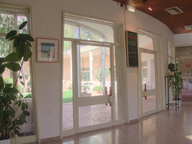
\includegraphics[width=\textwidth]{figures/chapter2/tmos44/44_drago03.png}
    \caption{Drago et al. ~\cite{drago2003adaptive}}
\end{subfigure}\hfill
\begin{subfigure}[b]{0.33\textwidth}
    \centering
    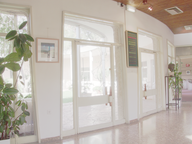
\includegraphics[width=\textwidth]{figures/chapter2/tmos44/44_mai11.png}
    \caption{Mai et al. ~\cite{mai2010optimizing}}
\end{subfigure}\hfill
\begin{subfigure}[b]{0.33\textwidth}
    \centering
    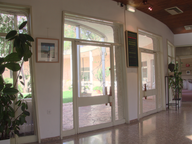
\includegraphics[width=\textwidth]{figures/chapter2/tmos44/44_reinhard02.png}
    \caption{Reinhard et al. (local) ~\cite{reinhard2002photographic}}
\end{subfigure}\\
\begin{subfigure}[b]{0.33\textwidth}
   \centering
    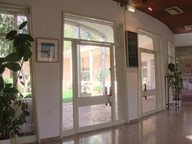
\includegraphics[width=\textwidth]{figures/chapter2/tmos44/44_reinhard02_global.png}
    \caption{Reinhard et al.(global) ~\cite{reinhard2002photographic}}
\end{subfigure}\hfill
\begin{subfigure}[b]{0.33\textwidth}
    \centering
    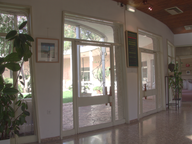
\includegraphics[width=\textwidth]{figures/chapter2/tmos44/44_durand02.png}
    \caption{Durand \& Dorsey~\cite{durand2002fast}}
\end{subfigure}\hfill
\begin{subfigure}[b]{0.33\textwidth}
    \centering
    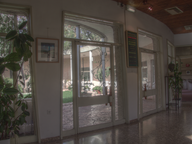
\includegraphics[width=\textwidth]{figures/chapter2/tmos44/44_mantiuk06.png}
    \caption{Mantiuk et al.~\cite{mantiuk2006perceptual}}
\end{subfigure}\\
\begin{subfigure}[b]{0.33\textwidth}
    \centering
    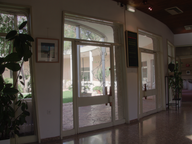
\includegraphics[width=\textwidth]{figures/chapter2/tmos44/44_reinhard05.png}
    \caption{Reinhard \& Devlin~\cite{reinhard2005dynamic}}
\end{subfigure}\hfill
\begin{subfigure}[b]{0.33\textwidth}
    \centering
    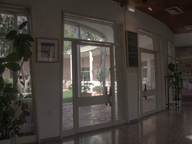
\includegraphics[width=\textwidth]{figures/chapter2/tmos44/44_fattal02.png}
    \caption{Fattal et al.~\cite{durand2002fast}}
\end{subfigure}\hfill
\begin{subfigure}[b]{0.33\textwidth}
    \centering
    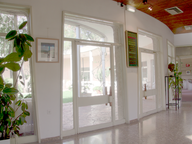
\includegraphics[width=\textwidth]{figures/chapter2/tmos44/44_mantiuk08.png}
    \caption{Mantiuk et al.~\cite{mantiuk2008display}}
\end{subfigure}\hfill
\begin{subfigure}[t]{\textwidth}
\centering
    \begin{subfigure}[t]{0.33\textwidth}
    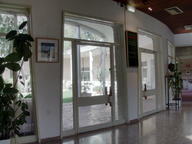
\includegraphics[width=\textwidth]{figures/chapter2/tmos44/44_ferradans11.png}
    \caption{Ferradans et al.~\cite{ferradans2011analysis}}
\end{subfigure}\hspace{-1pt}
\begin{subfigure}[t]{0.33\textwidth}
    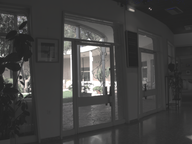
\includegraphics[width=\textwidth]{figures/chapter2/tmos44/44_pattanaik00.png}
    \caption{Pattanaik et al.~\cite{pattanaik2000time}}
\end{subfigure}\hfill
\end{subfigure}
%\\
%\begin{subfigure}[b]{0.33\textwidth}
%    \centering
%    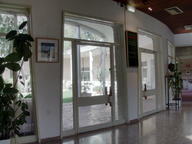
\includegraphics[width=\textwidth]{figures/chapter2/tmos44/44_ferradans11.png}
%    \caption{Ferradans et al.~\cite{ferradans2011analysis}}
%\end{subfigure}\hspace{-1pt}
%\begin{subfigure}[b]{0.33\textwidth}
%    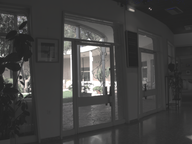
\includegraphics[width=\textwidth]{figures/chapter2/tmos44/44_pattanaik00.png}
%    \caption{Pattanaik et al.~\cite{pattanaik2000time}}
%\end{subfigure}\hfill
\caption{Tone mapping results for the "Belgium House" HDR image (image courtesy of Dani Lischinski) with different tone mapping operators. Note that pfstools~\cite{HDRGallery} implementation is used with default parameters.}
\label{fig:tmos}
\end{figure}

\section{Image Similarity}

Traditionally, image similarity is measured by measuring the distance between hand crafted features extracted from each image. These hand crafted features include simple descriptors such as color/luminance histograms, or improved ideas, including histogram of oriented gradients~\cite{dalal2005histograms}. GIST~\cite{oliva2001modeling}, SIFT~\cite{lowe2004distinctive}, SURF~\cite{bay2006surf}. These features are compared using several types of distance metrics. Recently, deep convolutional neural networks (DCNNs) became the state of art for image classification. Starting with AlexNet~\cite{krizhevsky2012imagenet} and followed by deeper networks such as VGG~\cite{simonyan2014very}, GoogleNet\cite{szegedy2015going}, and ResNet~\cite{he2016deep}, DCNNs started to perform near human level success for image classification. Their success lead to use feature vectors that have been obtained from DCNNs for image retrieval~\cite{wan2014deep,gordo2016deep,noh2017large,radenovic2018fine}. Unlike previous approaches that are based on hand-crafted features, DCNNs learn the feature vector itself directly from the image. 

The similarity between deep learning features can be calculated directly with euclidean or cosine distance without any learning, or can be learned. \cite{frome2007image}, \cite{mcfee2010metric}, \cite{liang2016optimizing} and  OASIS\cite{chechik2010large} are famous similarity learning techniques, that can be classified linear metric learning. These works proposed to work on hand-crafted image features but shown in \cite{wan2014deep} that can also work with deep features. The second group of metric learning is nonlinear metric learning methods, that learn similarity metric directly with deep neural network architectures\cite{pinheiro2018unsupervised}. Siamese\cite{chopra2005learning}\cite{bell2015learning} and triplet\cite{wang2014learning} \cite{arandjelovic2016netvlad} architectures minimizes the classification loss function while a more recent study \cite{garcia2019learning} proposes similarity network architecture to obtain similarity score by minimizing a ranking loss function.

One major drawback of using DCNNs is the need for using very large labeled datasets for training, which is difficult to obtain or not available at all for most problem domains. Transfer learning~\cite{yosinski2014transferable} aims to solve this problem by using pretrained networks on large scale datasets such as ImageNet~\cite{russakovsky2015imagenet}. The basic method is to give the images to the pre-trained network and use the output of the last fully connected layers as feature vectors~\cite{donahue2014decaf,wan2014deep} -- an approach that is also adopted in this thesis.

Visual similarity is a perceptual phenomenon without ground-truth data. This makes collecting data using crowdsourcing experiments valuable. Indeed, there are several crowdsourcing-based works~\cite{lun2015elements,saleh2015learning,kleiman2016toward} that address shape or style similarity problems and conduct user experiments to either derive or validate models. 

Of most related to our work are two similarity studies that also employ subjective experiments. Among these, in Rogowitz et al.~\cite{rogowitz1998perceptual}, human participants are asked to judge image similarity using two different experiments: one involving printouts of images (called table scaling) and the other using a computer based comparison (called computer scaling). These results are compared with computational similarity approaches~\cite{frese1997methodology} and simple CIELAB histograms. It was found that both table and computer scaling yield similar results and color is a major factor influencing similarity for human observers.

In another study~\cite{neumann2006image}, user experiments are conducted to evaluate the relationship between an image-indexing system and perceived similarity in an LDR setting. The tested image indexing system is based on basic properties of early stages of human vision -- chromaticity, luminance, and texture. Two-alternative forced-choice (2AFC) method is used for all experiments. Three images are shown to the observer, the query image and two test images. Of these two images one image is called the target and the other the distractor. These images are selected based on the rankings obtained from the image-indexing system. Then the correlation between the users' preference and index rank is investigated. First, each index, chromaticity, luminance, and texture are calculated separately. From these indexes chromaticity is found to give the best results. Then for the second experiment, combinations of the indexes are evaluated. The combination of chromaticity and texture indices are found to give better results than chromaticity alone and the combination of all indices are found to give the best result.

As mentioned above, although visual image similarity is an extensively studied subject~\cite{liu2007survey}, to our knowledge there is no study that directly addresses this problem for HDR images. Thus, understanding the nature of image similarity for HDR images and developing an objective similarity measure is the primary goal of this thesis. 